\section{Simulations}

\subsection{Constant length pendulum}

In this first part, we will consider the case where \(\alpha=0\) and \(d=0\), that is the length of the pendulum remains constant \(\ell(t)=L\). This corresponds to the situation analysed in \autoref{sec:analytic:constant_length}. Using a small initial angle of \(\theta_0=10^{-10}\) and no initial speed, a convergence study of the final angle and angular speed of the velocity-Verlet method was done. Comparing the final position obtained numerically with the analytical result, we obtain an error on the final position. The results in \autoref{fig:numeric_convergence_small_angle} show that the order of convergence of this method, for these initial conditions, are 4 and 2 for the position and speed respectively.

\begin{figure}[h]
    \centering
    \begin{subfigure}{0.48\linewidth}
        \centering
        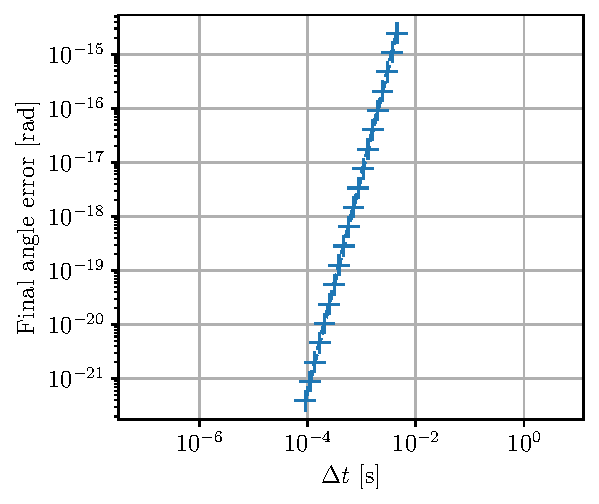
\includegraphics[width=\linewidth]{figures/no_excitation_pos_conv.pdf}
        \caption{Position (angle of pendulum)}
    \end{subfigure}
    \begin{subfigure}{0.48\linewidth}
        \centering
        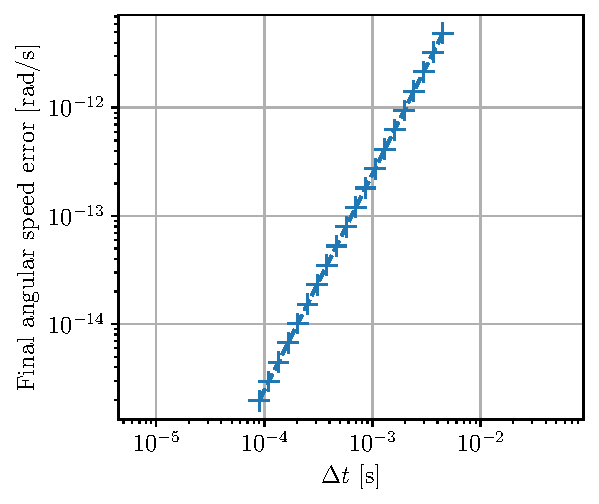
\includegraphics[width=\linewidth]{figures/no_excitation_vel_conv.pdf}
        \caption{Angular velocity}
    \end{subfigure}
    \caption{Numeric convergence of different variables for initial conditions \(\theta_0=10^{-10}\), \(\dot\theta_0=0\) and simulated until \(t_\textrm{fin} \approx 2.69\), corresponding to 3 periods of oscillation.}
    \label{fig:numeric_convergence_small_angle}
\end{figure}

Varying the initial angle \(\theta_0\) between \(0\) and \(\pi\) allows us to get larger movement from the pendulum, as shown in \autoref{fig:oscillations_time}. The angular frequency was extracted by looking at the time elapsed between the starting condition and the time it takes for two sign changes in angular speed (otherwise we would be measuring a half-period). Writing that time as \(T\), the period of oscillation, we get the angular frequency \(\Omega = \frac{2\pi}{T}\). The results are shown in \autoref{fig:angular_frequency}. These results are coherent with the physical reality, as a larger angle should correspond to a longer oscillation period than a smaller angle. It is interesting to note that the angular frequency does not change linearly, which is consistent with the results measured in the lab: small angles have less effect than large angles.

\begin{figure}[h]
    \centering
    \begin{subfigure}{0.48\linewidth}
        \centering
        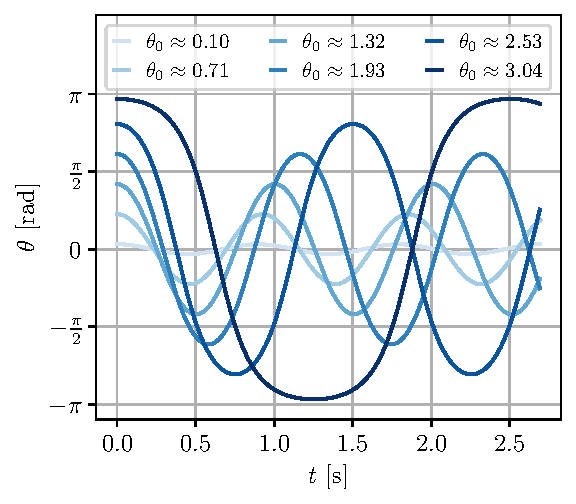
\includegraphics[width=\linewidth]{figures/oscillations_trajectory.pdf}
        \caption{Time evolution}
        \label{fig:oscillations_time}
    \end{subfigure}
    \begin{subfigure}{0.48\linewidth}
        \centering
        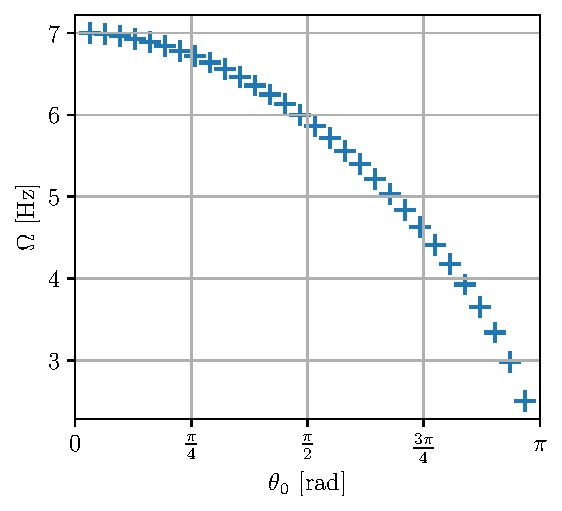
\includegraphics[width=\linewidth]{figures/angular_frequency.pdf}
        \caption{Angular frequency}
        \label{fig:angular_frequency}
    \end{subfigure}
    \caption{Time evolution and angular frequency for multiple starting angles (\(n_\textrm{steps}=10000\))}
\end{figure}


\subsection{Decreasing length pendulum}
\begin{wrapfigure}{h}{0.5\linewidth}
    \centering
    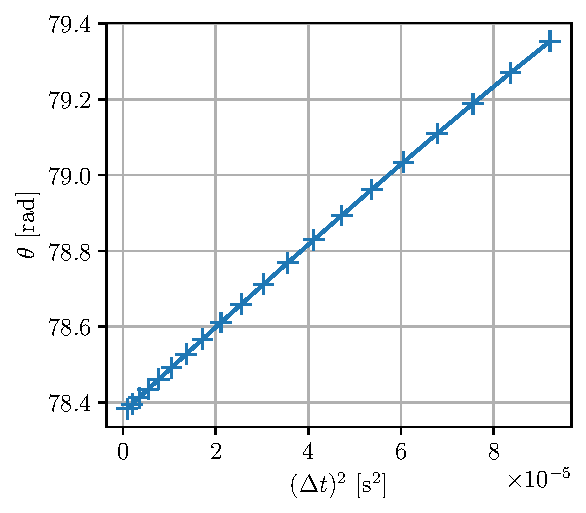
\includegraphics[width=\linewidth]{figures/converg_retraction.pdf}
    \caption{Convergence of the velocity-Verlet algorithm for a pendulum with decreasing length, initial conditions: $\theta_0 = 0.5$, $\dot{\theta}_0 = 0$ \si{\per\second}}
    \label{fig:conv_retract}
\end{wrapfigure}
The next simulations were run with conditions $\alpha=-0.02$ \si{\meter\per\second} and $d=0$ \si{\meter} and up to $t_\textrm{fin}=0.96L/|\alpha|$ in order to show the behavior of the mass when its rod has a length decreasing almost to 0. First a convergence analysis was done to determine the characteristics of the algorithm used. The various final positions for a given time step $\Delta t$ are shown in \autoref{fig:conv_retract}. Taking the time step squared show the points aligning which indicates that the velocity-Verlet algorithm converged in order 2 for this simulation.

The first step in studying this system is understanding conceptually how it behaves. As shown in \autoref{fig:retract_time} the oscillations remain low until close to the end of the simulation, corresponding to a very short rod for the pendulum, where they explode. The values in radians going up to 80 show that in the simulation the pendulum stops oscillating aroung its stable equilibrium and rather does complete rotations around the center $\mathcal{O}$. This is coherent with the fact that it will have not only gained mechanical energy with the work from the tension $T$ but as the rod gets shorter less energy is required to do a complete rotation. The phase space in \autoref{fig:retract_phase} also shows the small oscillations followed by an explosion towards higher values of $\theta$ and $\dot\theta$. A final point on these plots is that we can see the algorithm is very consistent for small time steps with almost no visible differences between the various time steps represented.
\begin{figure}[h]
    \centering
    \begin{subfigure}{0.48\linewidth}
        \centering
        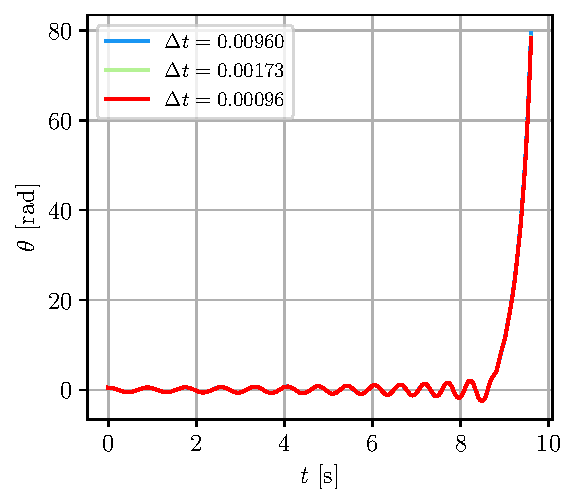
\includegraphics[width=\linewidth]{figures/traj_retraction.pdf}
        \caption{Time evolution}
        \label{fig:retract_time}
    \end{subfigure}
    \begin{subfigure}{0.48\linewidth}
        \centering
        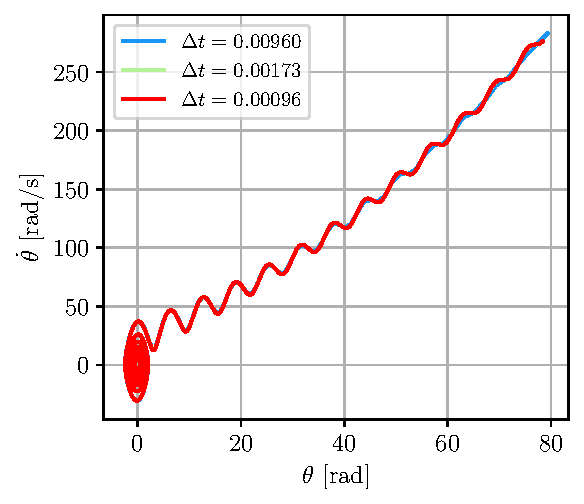
\includegraphics[width=\linewidth]{figures/phase_retraction.pdf}
        \caption{Phase space}
        \label{fig:retract_phase}
    \end{subfigure}
    \caption{Time evolution and phase space of a pendulum with decreasing length for various time steps, initial conditions: $\theta_0 = 0.5$, $\dot{\theta}_0 = 0$ \si{\per\second}}
\end{figure}

\begin{figure}[h]
    \centering
    \begin{subfigure}{0.48\linewidth}
        \centering
        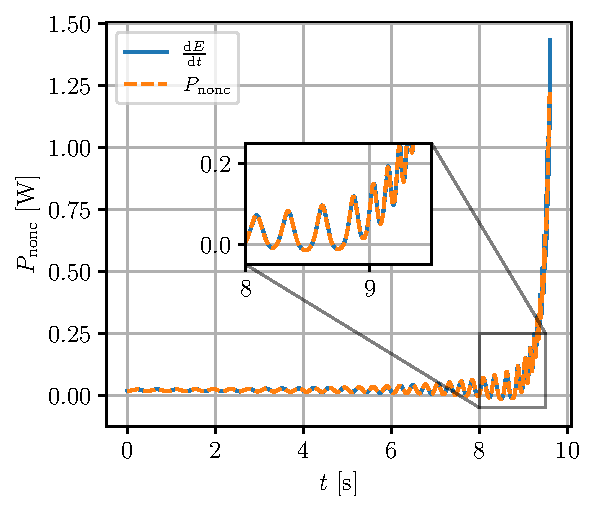
\includegraphics[width=\linewidth]{figures/retract_power.pdf}
        \caption{Power}
        \label{fig:retract_power}
    \end{subfigure}
    \begin{subfigure}{0.48\linewidth}
        \centering
        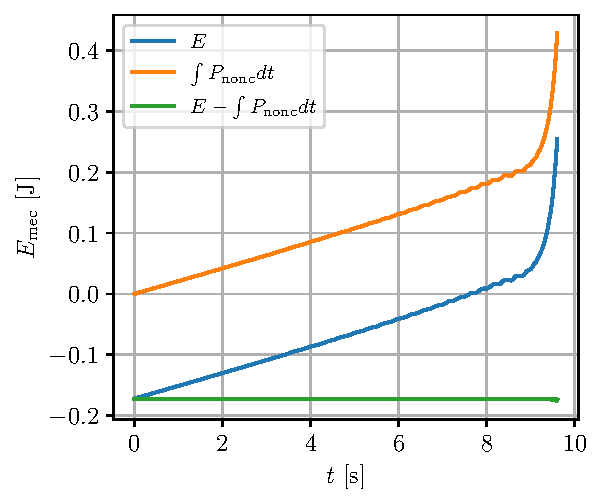
\includegraphics[width=\linewidth]{figures/retract_energy.pdf}
        \caption{Energy}
        \label{fig:retract_energy}
    \end{subfigure}
    \caption{Theorem of mechanical energy for a pendulum with decreasing length; initial conditions: $\theta_0 = 0.5$, $\dot{\theta}_0 = 0$ \si{\per\second}; $n_\textrm{steps}=2000$}
\end{figure}
A final physical point of interest is the energy of the system. We want to verify if the algorithm respects the theorem of mechanical energy $\dd E_{mec}/\dd t$. The \autoref{fig:retract_energy} and \autoref{fig:retract_power} show that this theorem is perfectly verified in this simulation. The \autoref{fig:retract_power} in particular illustrates that the variation of the energy in time, calculated through centered differences, is exactly the power. This can also be illustrated by integrating the power, this is done by summing the small $\dd P = P_\mathrm{nonc} \dd t$, and showing as in \autoref{fig:retract_energy} that substracting it to the energy gives a constant.


\subsection{Oscillating length pendulum}
The final case study concerns the conditions $\alpha=0$ \si{\meter\per\second}, $d=0.01$ \si{\meter} and $\omega = 2\omega_0 = 2\sqrt{g/L}$ as calculated in \autoref{sec:analytic:constant_length}.

\begin{wrapfigure}{h}{0.5\linewidth}
    \centering
    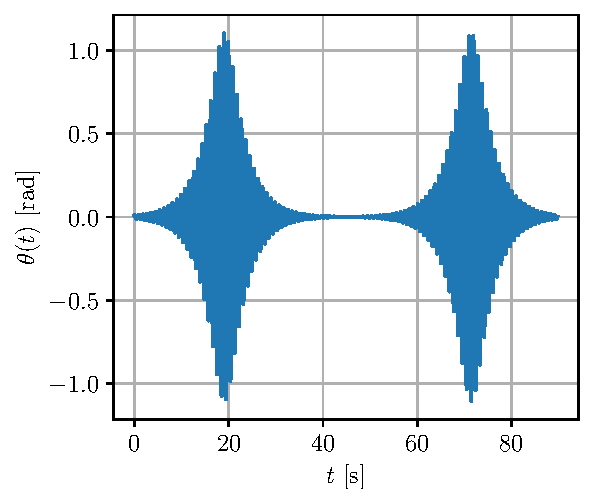
\includegraphics[width=\linewidth]{figures/excitation_smol_traj.pdf}
    \caption{Time evolution of an oscillator excited through varying length of its rod, initial conditions: \mbox{$\theta_0 = 0.01$}, $\dot{\theta}_0 = 0$ \si{\per\second}}
    \label{fig:excit_smol}
\end{wrapfigure}
Taking small oscillations, $\theta_0 = 0.01$, we can illustrate the behavior of an excited oscillator as shown in \autoref{fig:excit_smol}. This simulation was run for 200 periods of the oscillation of the length $T_\mathrm{excit} = 2\pi / \omega$. This corresponds numerically to two large oscillations of the amplitude of the smaller oscillations. This behavior indicates that the excitations increase the energy to a maximum giving larger oscillations and then start working against it to bring it back to a minimum.

An interesting feature of this new system is the chaotic behavior it can present. By taking larger oscillations we first need to analyse the convergence of our algorithm in this new chaotic system. As can be seen in \autoref{fig:chaos_10_per} and \autoref{fig:chaos_20_per} the velocity-Verlet algorithm still converges correctly in order 2 for 10 periods of excitation. However after too many excitations, here 20 periods, with a decreasing $\Delta t$ the final position does not converge to a single value in any polynomial order. It oscillates slightly due to the chaotic nature of the system.
\begin{figure}[h]
    \centering
    \begin{subfigure}{0.48\linewidth}
        \centering
        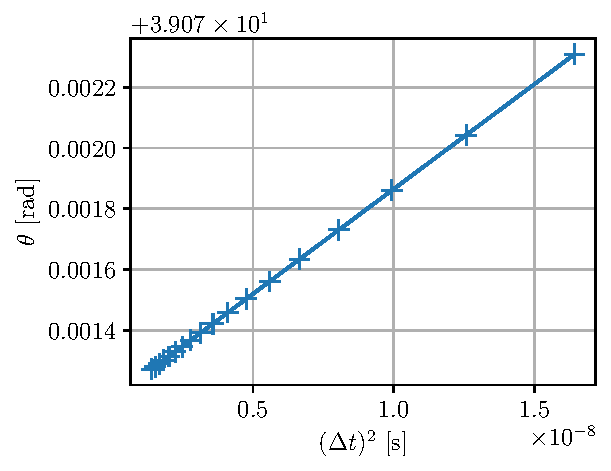
\includegraphics[width=\linewidth]{figures/chaos1_10_periods_conv.pdf}
        \caption{10 periods}
        \label{fig:chaos_10_per}
    \end{subfigure}
    \begin{subfigure}{0.48\linewidth}
        \centering
        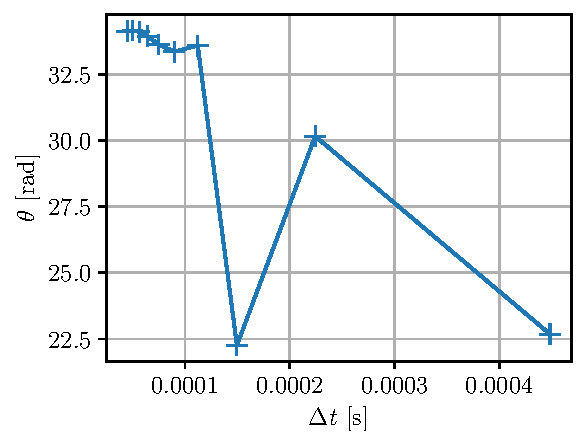
\includegraphics[width=\linewidth]{figures/chaos1_20_periods_conv.pdf}
        \caption{20 periods}
        \label{fig:chaos_20_per}
    \end{subfigure}
    \caption{Convergence of the velocity-Verlet algorithm for a chaotic system and different numbers of periods of excitation}
\end{figure}

To further illustrate the chaos in this system we can show the strong dependence on initial conditions. The distance represented in \autoref{fig:lyapounov} was calculated with the formula:
\begin{equation}
    \delta(t) = \sqrt{\omega_0^2(\theta_1(t) - \theta_2(t))^2 + (\dot\theta_1(t) - \dot\theta_2(t))^2}
\end{equation}
It represents a distance between two trajectories during 40 periods of excitation, $\theta_1$ and $\theta_2$, corresponding respectively to the initial conditions $\theta_{0,1} = 0$, $\dot\theta_{0,1} = 15$ \si{\per\second} and $\theta_{0,2} = 10^{-6}$, $\dot\theta_{0,2} = 15$ \si{\per\second}. These two very close initial conditions give diverging trajectories as illustrated by the growth of the distance $\delta$. This represents an exponential growth of the divergence with an exponent, the exponent of Lyapounov: $\lambda \approx 0.58$. This allows to characterise the chaos of this system by knowing the rate of growth of the divergence of trajectories with similar starting conditions.

\begin{figure}[H]
    \centering
    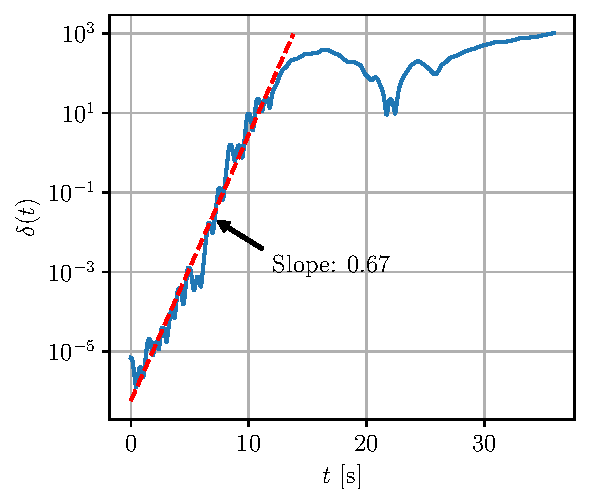
\includegraphics[width=0.6\linewidth]{figures/lyapounov.pdf}
    \caption{Distance in the phase space between two chaotic trajectories for an oscillator with varying length, indication of the Lyapounov exponent}
    \label{fig:lyapounov}
\end{figure}



\subsection{Poincaré map}
The same chaotic system can be sampled more clearly through a Poincaré map. To achieve this we run the simulation with a set number of steps $n_\mathrm{steps} = 1000$ per period and we sample the phase space at every period. The \autoref{fig:poincaré} shows the results for 8 different given initial conditions and 30 000 periods. We see that for values of $\theta_0$ up t0 $\pi / 2$ and $\dot\theta_0 = 0$ \si{\per\second}, or a sufficiently small $\dot\theta_0$ to have a similar level of energy here 2 \si{\per\second}, we have a stable, constant poincaré map representing a non-chaotic system. For these conditions the system will show a behavior similar to the one obtained in \autoref{fig:excit_smol}. Above this treshold of initial energy the system becomes chaotic and samples the same shape shown by two different initial conditions in \autoref{fig:poincaré}.
\begin{figure}[h]
    \centering
    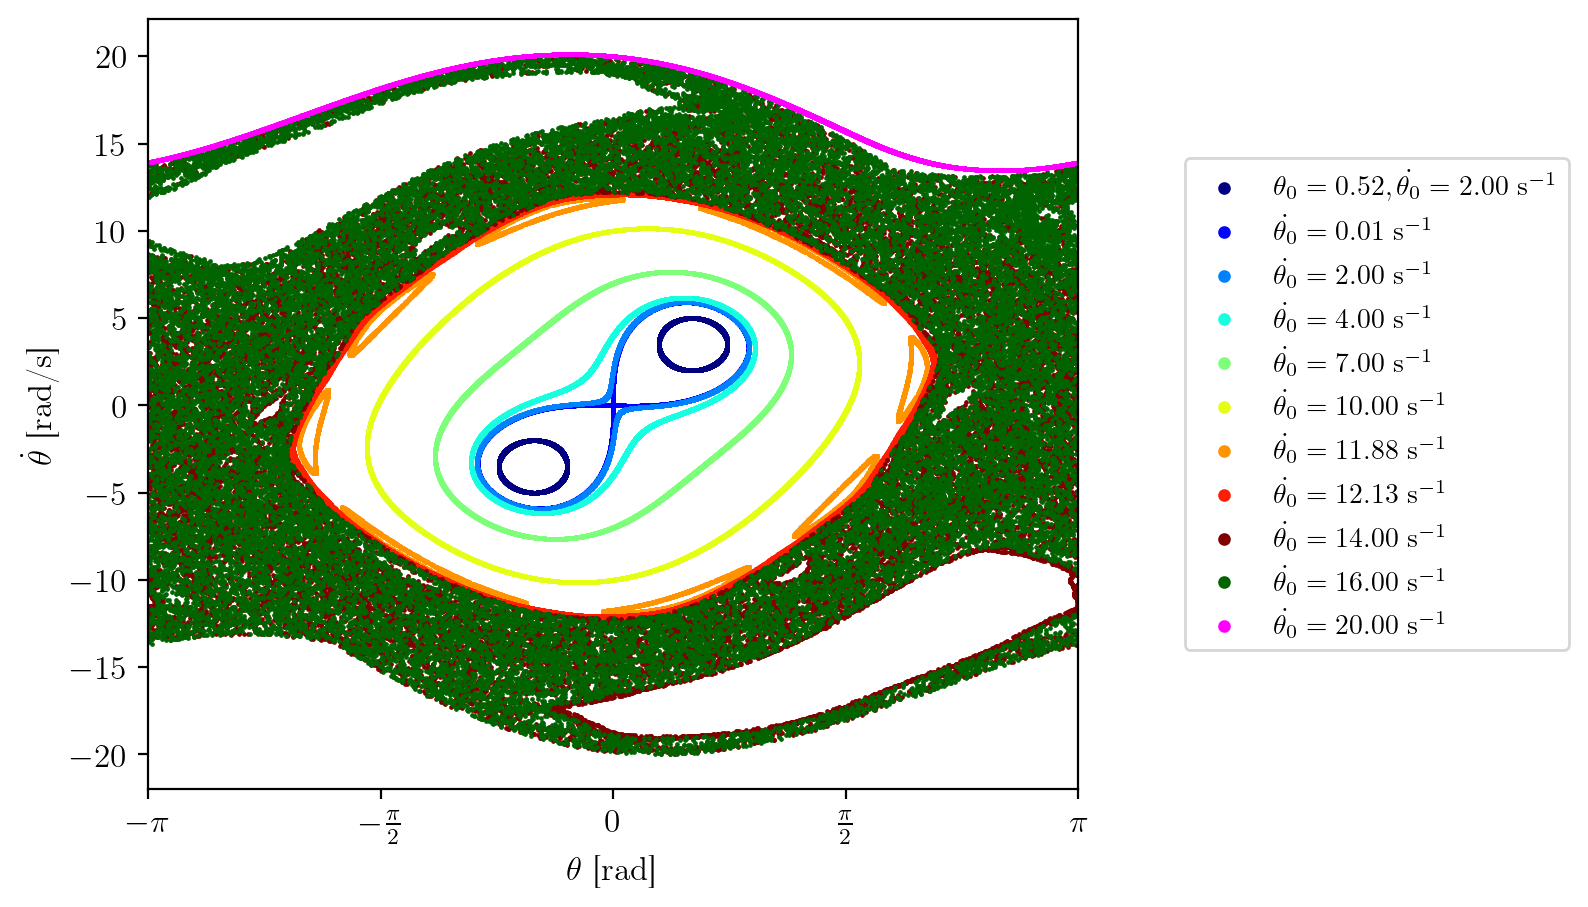
\includegraphics[width=\linewidth]{figures/poincare_overkill.png}
    \caption{Poincaré map of a chaotic system, a pendulum with varying length, for various initial conditions. \(\theta_0=0\) unless said otherwise. (\(n_\textrm{steps}=1000\), \(N=30000\) periods of excitation)}
    \label{fig:poincaré}
\end{figure}





